\FloatBarrier
Precision miniaturized sensors have become an increasingly relevant technology over 
recent decades, finding applications in navigation, medical diagnostics, geophysical 
surveying, and fundamental physics research \cite{lucivero2022}. 
The growing demand for 
compact, high-performance devices has driven the development of new fabrication 
techniques capable of producing smaller, more complex geometries while maintaining 
extreme gas purity, free of contaminants that could degrade sensor performance. 
Manufacturing such devices is inherently challenging: the internal cavities must be 
hermetically sealed to prevent outgassing or contamination, the interaction volume 
must be precisely defined to ensure reproducibility, and the cell must accommodate 
optical access from multiple directions to support the beam geometries required by 
techniques such as multipass cells, dual-beam, or cavity-enhanced sensing 
\cite{lucivero2022}. Traditional fabrication strategies, such as MEMS-based anodic 
bonding, offer excellent scalability but 
are fundamentally limited to planar geometries and restricted optical access.
Photolithographic approaches, while capable of producing 
nanostructured vapor cells, share the same limitation of planar bonding strategies 
\cite{cutler2020}.

A Laser-Written Vapor Cell (LWVC) addresses these limitations by exploiting the 
three-dimensional structuring capabilities of Femtosecond Laser Writing (FLW), enabling 
arbitrary buried geometries within a monolithic transparent substrate 
\cite{lucivero2022}. The complete fabrication workflow is illustrated in 
Fig.~\ref{fig:lwvc_fabrication} and consists of four main steps, each of which 
contributes to the precision and hermeticity of the final device, as described below 
and discussed in detail in the following sections.
\begin{figure}[h]
\centering
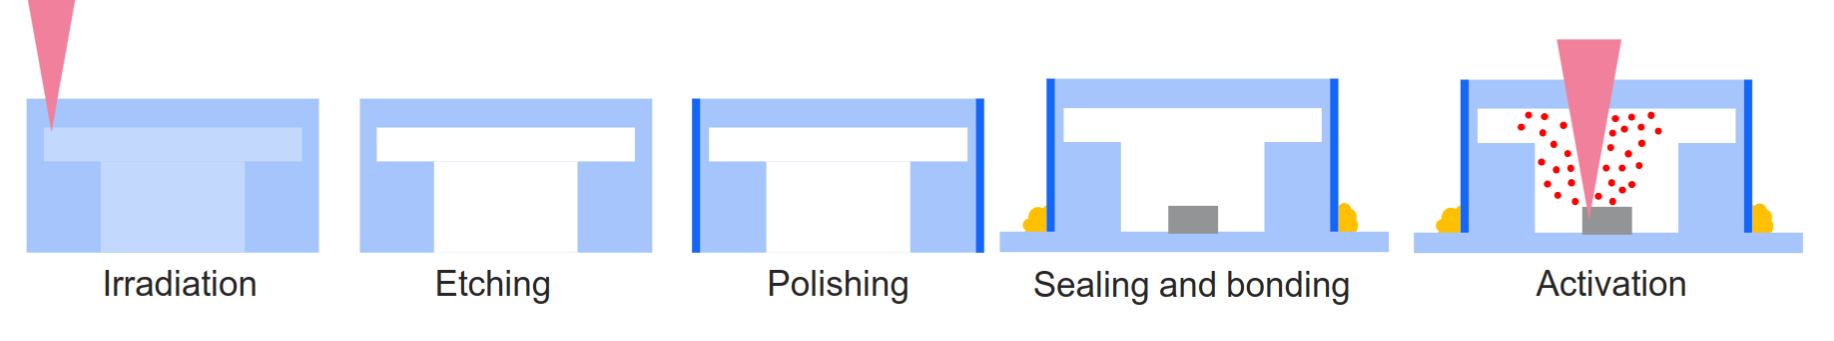
\includegraphics[width=1\linewidth]{Images/lwvc_process.png}
\caption{Fabrication worklow of a Laser-Written Vapor Cell.
Steps (1-2) describe the FLICE process. In step (3) NEG dispenser placement and
bonding are performed. Activation is illustrated by step (4). Adapted from \cite{lucivero2022}.}
\label{fig:lwvc_fabrication}
\end{figure}
\subsection*{Step 1: Femtosecond Laser Writing and Chemical Etching (FLICE)}
The first step employs the so-called FLICE technique (Femtosecond Laser Irradiation 
followed by Chemical Etching), a two-stage maskless microfabrication process 
\cite{lucivero2022}. An ultrafast laser beam is tightly focused inside the bulk of a 
fused silica substrate, inducing the local formation of self-oriented nanogratings 
through nonlinear absorption. Because the material modification is confined to the 
laser focal spot, arbitrary three-dimensional patterns can be inscribed with 
micrometric resolution and without any lithographic mask. In the second stage, the 
substrate is immersed in a hydrofluoric acid solution, which selectively removes the 
irradiated material, leaving behind hollow channels and reservoirs with the desired 
geometry. The non-irradiated fused silica remains unaffected, preserving the 
monolithic integrity of the substrate and its broad optical transparency window ---a 
key advantage for spectroscopic characterization of the gas content. This maskless 
approach enables geometries that are inaccessible to planar bonding or 
photolithographic techniques, including fully buried sensing channels and multi-sided 
optical access. The FLICE process and its optimization for LWVC fabrication are 
further discussed in Section~\ref{sec:flice}.
\subsection*{Step 2: Placement of the Non-Evaporable Getter Dispenser}
Once the internal cavities have been formed, a pill of non-evaporable getter (NEG) 
material is placed inside the reservoir cavity of the fused silica structure 
\cite{lucivero2022}. \gls{NEG} materials serve a dual function: upon thermal activation, 
they simultaneously release the alkali metal vapor required 
for atomic sensing, and absorb residual buffer gases such as nitrogen. This dual 
action enables the production of cells with sub-atmospheric buffer gas pressures 
without the need for a vacuum apparatus, greatly simplifying the manufacturing 
process while maintaining the gas purity essential for high-precision applications. 
The ability to control the buffer gas pressure post-sealing ---by adjusting the duration 
of getter heating or by pre-filling with controlled fractions of ungetterable gases 
such as argon--- offers an additional degree of freedom for optimizing sensor 
performance \cite{lucivero2022}.
\subsection*{Step 3: Sealing and Bonding}
After the dispenser has been placed, the cell must be hermetically sealed to prevent 
contamination and ensure long-term stability. The sealing is performed inside a 
controlled-atmosphere chamber filled with nitrogen containing very low amounts of 
O\textsubscript{2}, thereby preventing the trapping of reactive oxygen inside the 
cell \cite{lucivero2022}. The choice of bonding method is critical, as it directly 
affects hermeticity, thermal stability, and compatibility with the cell's optical 
coatings and internal components.

Bonding glass and crystal presents unique engineering challenges due to the 
material's non-porous nature, extreme smoothness, and high surface energy. In 
industrial applications, several established methods are traditionally deployed to 
ensure structural integrity and optical clarity. For instance, UV-curing adhesives 
utilize one-component resins that polymerize rapidly upon ultraviolet exposure, 
offering precise and optically transparent joints since their refractive index can 
be matched to the substrate \cite{paschotta2023}. Alternatively, traditional 
anodic bonding eliminates intermediate layers by heating the substrates to 
$300^{\circ}\text{C}$--$500^{\circ}\text{C}$ while applying a high voltage 
($\approx 1~\text{kV}$), which drives ion migration and generates a powerful 
electrostatic attraction to form a permanent chemical bond \cite{wallis1974}. More 
recently, laser microwelding has been introduced to locally melt and fuse glass 
interfaces using a focused beam, achieving a bond without high global temperatures 
or additional adhesives \cite{wlodarczyk2019}.

Each of these traditional approaches, however, presents distinct trade-offs in the 
context of \gls{MEMS} and vapor cell manufacturing. Adhesive-based bonding remains 
highly problematic for high-precision atomic devices due to resin outgassing and 
subsequent alkali vapor contamination \cite{knapkiewicz2018}, as well as poor 
long-term hermeticity \cite{karlen2018}. To circumvent chemical contamination, 
adhesive-free alternatives like anodic bonding achieve excellent hermeticity, but 
their reliance on elevated global temperatures induces severe thermal stress and 
renders them incompatible with temperature-sensitive optical or anti-relaxation 
coatings \cite{wang2025}. 

To overcome these limitations, advanced techniques such as femtosecond laser 
welding ---an evolution of standard laser microwelding \cite{wlodarczyk2019}--- 
and \textit{Optical Contact Bonding} \cite{gosele2006} have emerged as the most viable modern, 
adhesive-free paradigms for glass microfabrication. While femtosecond laser 
welding successfully 
eliminates global heating by fusing the interfaces through highly localized absorption, 
it demands meticulous management of intense thermal gradients to mitigate residual 
stress or micro-cracking along the weld track. Alternatively, 
Optical Contact Bonding achieves a hermetic joint entirely at room temperature through 
intermolecular van der Waals and hydrogen-bond interactions between two ultra-flat, 
clean surfaces. 

While both modern techniques represent powerful 
solutions for vapor-cell encapsulation, this thesis focuses specifically on the 
development and optimization of the Optical Contact Bonding approach. This 
room-temperature method is fully compatible with the FLICE-based LWVC fabrication 
process and is discussed in comprehensive detail in 
Section~\ref{sec:optical_contact_bonding}.
\subsection*{Step 4: Getter Activation}
In the final step, the sealed cell is exposed to a focused laser beam directed at the 
NEG dispenser through the fused silica substrate. The laser locally heats the 
dispenser, triggering the release of alkali vapor into the sensing chamber and the 
simultaneous absorption of residual buffer gas \cite{lucivero2022}. Because the 
activation is performed optically and post-sealing, the cell does not need to be 
re-opened or placed in a vacuum system, preserving hermeticity throughout the entire 
process. The precise control of activation time and laser power allows the residual 
buffer gas pressure to be tuned, directly influencing key sensing parameters such as 
the spin coherence time and pressure-induced spectral broadening. The activation 
procedure and its effects on cell performance are discussed in 
Section~\ref{sec:neg_dispenser}.